\documentclass{article}\usepackage{graphicx, color}
%% maxwidth is the original width if it is less than linewidth
%% otherwise use linewidth (to make sure the graphics do not exceed the margin)
\makeatletter
\def\maxwidth{ %
  \ifdim\Gin@nat@width>\linewidth
    \linewidth
  \else
    \Gin@nat@width
  \fi
}
\makeatother

\definecolor{fgcolor}{rgb}{0.2, 0.2, 0.2}
\newcommand{\hlnumber}[1]{\textcolor[rgb]{0,0,0}{#1}}%
\newcommand{\hlfunctioncall}[1]{\textcolor[rgb]{0.501960784313725,0,0.329411764705882}{\textbf{#1}}}%
\newcommand{\hlstring}[1]{\textcolor[rgb]{0.6,0.6,1}{#1}}%
\newcommand{\hlkeyword}[1]{\textcolor[rgb]{0,0,0}{\textbf{#1}}}%
\newcommand{\hlargument}[1]{\textcolor[rgb]{0.690196078431373,0.250980392156863,0.0196078431372549}{#1}}%
\newcommand{\hlcomment}[1]{\textcolor[rgb]{0.180392156862745,0.6,0.341176470588235}{#1}}%
\newcommand{\hlroxygencomment}[1]{\textcolor[rgb]{0.43921568627451,0.47843137254902,0.701960784313725}{#1}}%
\newcommand{\hlformalargs}[1]{\textcolor[rgb]{0.690196078431373,0.250980392156863,0.0196078431372549}{#1}}%
\newcommand{\hleqformalargs}[1]{\textcolor[rgb]{0.690196078431373,0.250980392156863,0.0196078431372549}{#1}}%
\newcommand{\hlassignement}[1]{\textcolor[rgb]{0,0,0}{\textbf{#1}}}%
\newcommand{\hlpackage}[1]{\textcolor[rgb]{0.588235294117647,0.709803921568627,0.145098039215686}{#1}}%
\newcommand{\hlslot}[1]{\textit{#1}}%
\newcommand{\hlsymbol}[1]{\textcolor[rgb]{0,0,0}{#1}}%
\newcommand{\hlprompt}[1]{\textcolor[rgb]{0.2,0.2,0.2}{#1}}%

\usepackage{framed}
\makeatletter
\newenvironment{kframe}{%
 \def\at@end@of@kframe{}%
 \ifinner\ifhmode%
  \def\at@end@of@kframe{\end{minipage}}%
  \begin{minipage}{\columnwidth}%
 \fi\fi%
 \def\FrameCommand##1{\hskip\@totalleftmargin \hskip-\fboxsep
 \colorbox{shadecolor}{##1}\hskip-\fboxsep
     % There is no \\@totalrightmargin, so:
     \hskip-\linewidth \hskip-\@totalleftmargin \hskip\columnwidth}%
 \MakeFramed {\advance\hsize-\width
   \@totalleftmargin\z@ \linewidth\hsize
   \@setminipage}}%
 {\par\unskip\endMakeFramed%
 \at@end@of@kframe}
\makeatother

\definecolor{shadecolor}{rgb}{.97, .97, .97}
\definecolor{messagecolor}{rgb}{0, 0, 0}
\definecolor{warningcolor}{rgb}{1, 0, 1}
\definecolor{errorcolor}{rgb}{1, 0, 0}
\newenvironment{knitrout}{}{} % an empty environment to be redefined in TeX

\usepackage{alltt}
\IfFileExists{upquote.sty}{\usepackage{upquote}}{}


\begin{document}

\title{Williamstown Weather Package}
\author{Angel Zhou and Michaela Kane}
\maketitle

\section*{Introduction}

The Williamstown Weather package takes data tables of the temperatures
(in degrees Farenheit) of Williamstown, MA and, from the tables,
extracts the desired data sets of date and temperature and puts them
into a new data frame.

\section*{The Read Weather 1 Function}
The \verb+readWeather1+ function takes data formatted in a similar
manner to that of the table at
\verb+http://web.williams.edu/weather/100_history.php?type=Temperature+,
and creates a data frame directly comparing the date to the monthly
temperatures in Williamstown, MA from 1892 to 2010. This function
accepts as parameters the \verb+fileName+ (the name of the text file
of data to be used), the logical \verb+h+ value (if \verb+TRUE+, it
keeps the current header), and the \verb+dateFormat+ (what format the
date object should be read in as).
\\
\\
This is a box-and-whiskers plot of the monthly temperatures of
Williamstown, Massachusetts as recorded from January 1892 to December 2010.

\begin{knitrout}
\definecolor{shadecolor}{rgb}{0.969, 0.969, 0.969}\color{fgcolor}\begin{kframe}
\begin{alltt}
\hlfunctioncall{library}(lubridate)
\hlfunctioncall{library}(reshape)
\hlfunctioncall{library}(ggplot2)
x <- \hlfunctioncall{read.table}(\hlstring{"monthlyTemp.txt"}, header = TRUE)
y <- \hlfunctioncall{melt}(x, id = \hlstring{"Year"})
stringDates <- \hlfunctioncall{paste}(y$variable, y$Year, 20, sep = \hlstring{"/"})
Date <- \hlfunctioncall{as.Date}(stringDates, format = \hlstring{"%b/%Y/%d"})
y$Temperatures <- y$value
months <- \hlfunctioncall{months}(Date, abbr = TRUE)
months_fac = \hlfunctioncall{factor}(months, levels = month.abb)
y$Month <- \hlfunctioncall{sort}(months_fac)
weather1_5 <- \hlfunctioncall{ggplot}(y, \hlfunctioncall{aes}(Month, Temperatures)) + \hlfunctioncall{geom_boxplot}()
weather1_5
\end{alltt}
\end{kframe}
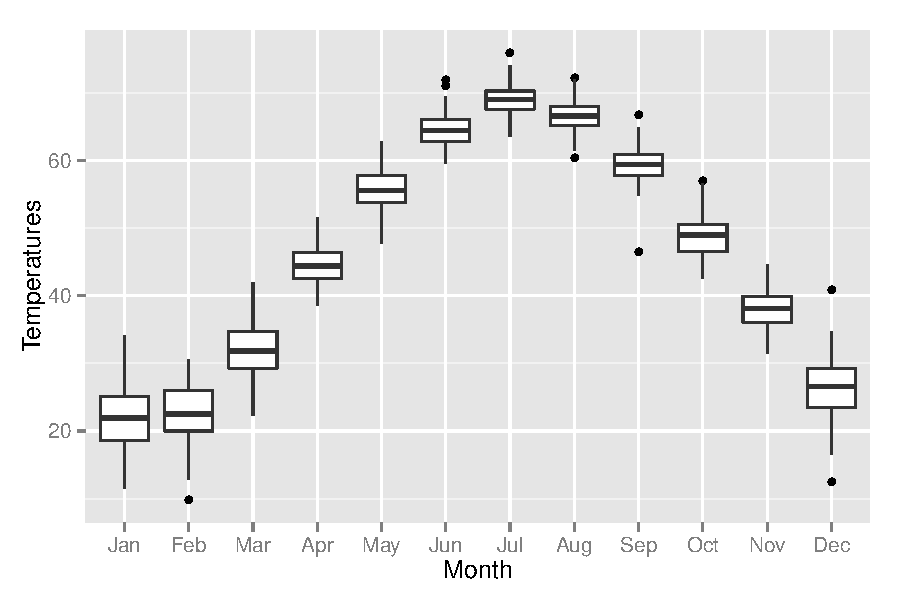
\includegraphics[width=\maxwidth]{figure/graph1_5} 

\end{knitrout}


\subsection*{Weather 2}
This takes the information from the following link:
\verb+http://web.williams.edu/weather/current_get_date_range.php?start=10_01_2005&end=6_10_2013&interval=24hours+
and creates a data frame of the date compared to the daily temperature
in degrees Farenheit of Williamstown, MA from 2005 to 2013.
\\
\\
This graph illustrates the average daily temperatures in degrees Celsius of
Williamstown, Massachusetts from 2005 to 2013.

\begin{knitrout}
\definecolor{shadecolor}{rgb}{0.969, 0.969, 0.969}\color{fgcolor}\begin{kframe}
\begin{alltt}
x <- \hlfunctioncall{read.table}(\hlstring{"dailyTemp1.txt"})
date <- x[, 1]
Temperature <- x[, 3]
dateTrim <- \hlfunctioncall{strtrim}(date, 10)
Date <- \hlfunctioncall{as.Date}(dateTrim)
y <- \hlfunctioncall{ggplot}(x, \hlfunctioncall{aes}(Date, Temperature))
y <- y + \hlfunctioncall{layer}(geom = \hlstring{"point"})
y
\end{alltt}
\end{kframe}
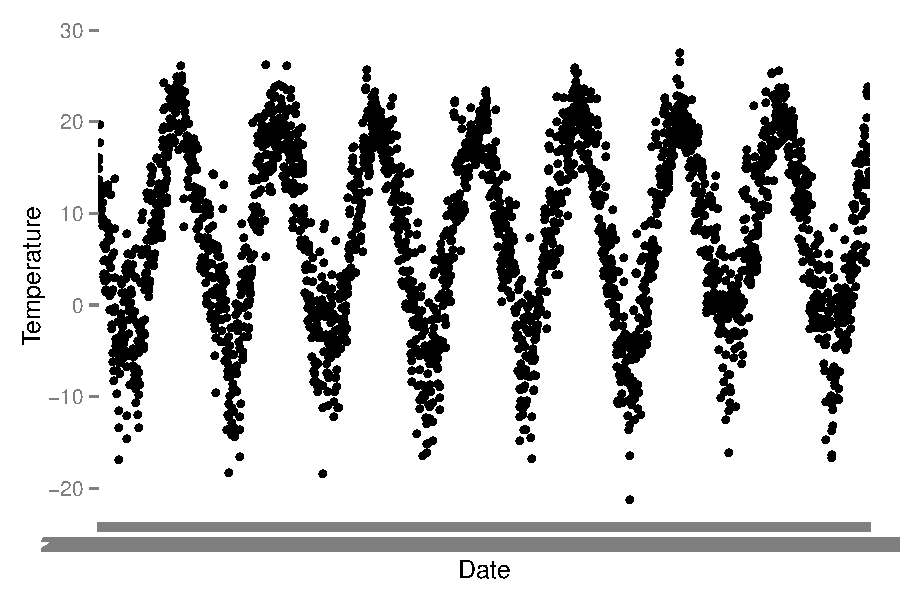
\includegraphics[width=\maxwidth]{figure/graph2} 

\end{knitrout}


\subsection*{Weather 3}
This takes the information from the following link:
 \verb+http://web.williams.edu/weather/archive_get_date_range.php?begin=1_01_1983&end=12_31_2007+
and creates a data frame of the date compared to the daily temperature
in degrees Farenheit of Williamstown, MA from 1983 to 2007.
\\
\\
This graph illustrates the average daily temperatures in degrees Celsius of
Williamstown, Massachusetts from 1983 to 2007.

\begin{knitrout}
\definecolor{shadecolor}{rgb}{0.969, 0.969, 0.969}\color{fgcolor}\begin{kframe}
\begin{alltt}
x <- \hlfunctioncall{read.table}(\hlstring{"dailyTemp2.txt"}, sep = \hlstring{"\textbackslash{}t"})
date <- x[, 1]
Temperature <- x[, 2]
dateTrim <- \hlfunctioncall{strtrim}(date, 10)
Date <- \hlfunctioncall{as.Date}(dateTrim)
y <- \hlfunctioncall{ggplot}(x, \hlfunctioncall{aes}(Date, Temperature))
y <- y + \hlfunctioncall{layer}(geom = \hlstring{"point"})
y
\end{alltt}


{\ttfamily\noindent\color{warningcolor}{\#\# Warning: Removed 1 rows containing missing values (geom\_point).}}\end{kframe}
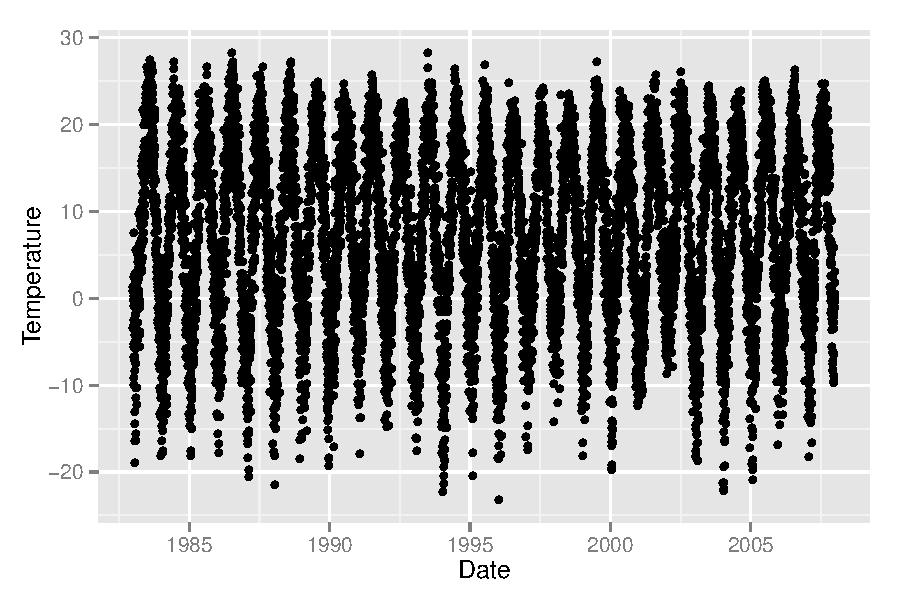
\includegraphics[width=\maxwidth]{figure/graph3} 

\end{knitrout}


\end{document}
